\documentclass[10pt,A4paper]{report}
\usepackage{amsmath}
\usepackage{microtype}	% Font improvement for pdflatex.
\usepackage{pgf}
\usepackage{tikz}
\usepackage{verbatim}
\usepackage{url}
\usepackage{hyperref}	% Clickable links to figures, references and urls.
\usepackage{float}		% Floating figure placement.
\usepackage{graphicx}
\usepackage{subfigure}

% Listings for wrapping code.
\usepackage{listings}
\lstset{breaklines=true}
\lstset{basicstyle=\small\ttfamily}

%Chapter 1 Introduction to FDTD
%1. 1D Equations
%2. 1D simple wave propagation
%3. Additive source, Stability, significance of Sc
%4. Boundary conditions
%Chapter 2 Dispersive Media
%5. 1D scatterer using Drude, epsilon=2
%6. 2D dispersive media, cylinder problem from Sadiku using Drude
%Chapter 3 Metamaterial Modelling using Dispersive Drude Model
%7. 1D DNG slab
%8. 2D DNG slab
%Chapter 4 FDTD Modelling of Lossless Cylindrical Cloak
%9. 2D FDTD implementation on Matlab
%10. 2D FDTD implementation on C++
%Chapter 5 GPU implementation of Lossless Cylindrical Cloak
%11. GPU considerations
%12. Implementation details
%13. Performance Analysis
%Conclusion

\begin{document}

% Title Page.
\input{FDTD_Title}

\begin{center}
\copyright Copyright\\[0.2in]
by\\[0.2in]
Attique Dawood\\[0.2in]
2012
\end{center}

\include{FDTD_Certification}

\tableofcontents
\listoffigures

\begin{abstract}
The Finite Difference Time-Domain method is a differential numerical technique for solving electromagnetic wave scattering problems. In order to model metamaterials with negative refractive index the standard algorithm is modified as implementation of the Drude dispersion model. Suitable values of plasma frequency ($\omega_p$) are chosen to model the metamaterial cloaking structure following the treatment of~\cite{Radial-Zhao}. The lossless case of electromagnetic cloak is implemented using a graphics processing unit (GPU). Simulation performance on Matlab, C++ and GPU is analysed.
\end{abstract}

\chapter{Introduction}
\section{Metamaterials}
Metamaterials are artificially manufactured with certain structural geometry. Electromagnetic waves passing through these metamaterials will act differently compared to naturally occurring materials. The behaviour of these metamaterials can change with frequency of incident EM wave and may exhibit negative values of permittivity and permeability under certain conditions. Some applications of metamaterials are perfect lens, invisibility cloak and novel antenna designs.

\section{Modelling Techniques}
Metamaterials can be modelled using analytical or numerical techniques. For problems with simple geometry and symmetry analytical methods give exact solution. For complex structures and irregular geometries, numerical techniques can be applied. Numerical techniques in electromagnetics are generally classified as either differential or integral. Examples of integral techniques are method of moment (MoM) and finite element method (FEM), whereas, finite difference time-domain (FDTD) is a differential technique.

\section{FDTD Modelling}
Integral techniques usually involve solving for unknowns in the problem domain. The number of unknowns determine the computational time required. On the other hand, FDTD is a brute force method that requires the whole problem domain to be discretized and stored in computer memory. Thus, the amount of computer memory is a constraint in the case of FDTD. Conceptually, FDTD is easier compared to integral methods.

\section{FDTD on Modern Hardware}
In recent times computer memory has become extremely cheap and a large number of complex problems can be readily and easily modelled using FDTD. Moreover, the recent advent of multi-core CPUs (central processing unit) favour methods and algorithms that can take advantage of parallel processing. Since, FDTD is a data parallel algorithm it is ideal in such a scenario.

In more recent times, GPUs (graphics processing units) with general purpose computing capabilities have arrived on the scene. These GPGPUs are in the order of 5--20 times faster than contemporary CPUs and are heavily multi-threaded. The goal of this thesis is to implement the classical cylindrical cloak on GPU using the FDTD method proposed in~\cite{Radial-Zhao}.

%\chapter{FDTD Modelling of Metamaterials}
\chapter{Introduction to Finite Difference Time-Domain Technique}

\section{The Yee Algorithm}

The original algorithm was proposed by K. S. Yee in 1966~\cite{Yee1966}. The derivatives in Faraday's Law and Ampere's Law are replaced with difference equations. The whole problem space is discretized and divided into cells such that electric and magnetic fields are staggered at half spatial steps in unit cell. By advancing the simulation in time, future values of electric and magnetic field components are computed using past values. This chapter gives provides a brief treatment of FDTD in 1D and 2D. Wave propagation in free space and with a homogeneous scatterer are discussed using conventional and dispersive FDTD methods.

\section{FDTD Update Equations in One Dimension (1D)}
Faraday's Law and Ampere's Law in differential form are given by:
\begin{equation}
\centering
\nabla \times \textbf{E} = - \dfrac{\partial \textbf{B}}{\partial t}
\label{Faraday's Law}
\end{equation}

\begin{equation}
\centering
\nabla \times \textbf{H} = \dfrac{\partial \textbf{D}}{\partial t}
\label{Ampere's Law}
\end{equation}

Assume electric field only has $x$-component, that is $E_x$, and magnetic field only has $y$-component $H_y$. The curl of electric field can be expanded as:
\begin{equation}
\centering
\nabla \times \textbf{E} = - \mu \dfrac{\partial H_y}{\partial t} \hat{y} = \left| \begin{array}{ccc} \hat{x} & \hat{y} & \hat{z} \\ \frac{\partial}{\partial x} & \frac{\partial}{\partial y} & \frac{\partial}{\partial z} \\ E_x & 0 & 0 \end{array} \right| = \dfrac{\partial E_x}{\partial z} \hat{y}
\label{Faraday's Law-Curl-Expansion}
\end{equation}
Similarly, the curl of magnetic field can be written as:
\begin{equation}
\centering
\nabla \times \textbf{H} = \epsilon \dfrac{\partial E_x}{\partial t} \hat{x} = \left| \begin{array}{ccc} \hat{x} & \hat{y} & \hat{z} \\ \frac{\partial}{\partial x} & \frac{\partial}{\partial y} & \frac{\partial}{\partial z} \\ 0 & H_y & 0 \end{array} \right| = - \dfrac{\partial H_y}{\partial z} \hat{x}
\label{Ampere's Law-Curl-Expansion}
\end{equation}
Rearranging terms,
\begin{equation}
\centering
\dfrac{\partial H_y}{\partial t} = - \dfrac{1}{\mu} \dfrac{\partial E_x}{\partial z}
\label{Faraday's Law-Curl-Expansion-1D}
\end{equation}
\begin{equation}
\centering
\dfrac{\partial E_x}{\partial t} = - \dfrac{1}{\epsilon} \dfrac{\partial H_y}{\partial z}
\label{Ampere's Law-Curl-Expansion-1D}
\end{equation}
These two scalar equations drive the FDTD algorithm. First, magnetic field is calculated using equation~\ref{Faraday's Law-Curl-Expansion-1D} and then electric field (equation~\ref{Ampere's Law-Curl-Expansion-1D}) is calculated from the magnetic field obtained in~\ref{Faraday's Law-Curl-Expansion-1D}. Electric and magnetic fields are staggered at half time steps. Similarly, magnetic and electric fields in space are also spaced at half spatial steps. The algorithm is normally referred to as a leap--frog scheme.

\begin{figure}[here]
\centering
%\includegraphics[width=\textwidth]{Algorithm.png}
\caption{The Yee algorithm. Figure taken from~\cite{JBSchneiderUFDTD}}
\label{Algorithm}
\end{figure}

By examining equations~\ref{Faraday's Law-Curl-Expansion-1D} and \ref{Ampere's Law-Curl-Expansion-1D} it can be intuitively observed that a wave with $E_x$ and $H_y$ components will propagate in $\hat{z}$ direction and space derivatives with respect to $z$ indicate variation of electric and magnetic fields in space along $z$-axis.

These equations need to be discretized before they can be implemented as a computer simulation. Both the time and space derivatives are discretized to obtain difference equations. Following the treatment in chapter 3 of~\cite{JBSchneiderUFDTD}, electric and magnetic fields as functions of time and space can be written as,
\begin{equation}
\centering
H_y (z,t)=H_y (k\Delta _z,n\Delta _t)=H^n_y[k]
\label{Hy-of-z_and_t}
\end{equation}
\begin{equation}
\centering
E_x (z,t)=E_x (k\Delta _z,n\Delta _t)=E^n_x[k]
\label{Ex-of-z_and_t}
\end{equation}
The final equations for electric and magnetic fields driving the FDTD algorithm are,
\begin{equation}
\centering
H^{n+\frac{1}{2}}_y \left[k+\frac{1}{2}\right]=H^{n-\frac{1}{2}}_y \left[k+\frac{1}{2}\right] + \dfrac{\Delta t}{\mu \Delta x} \left( E^{n}_x \left[k\right] - E^{n}_x \left[k+1\right] \right)
\label{Hy-1D-Simple-FDTD-Driver}
\end{equation}
\begin{equation}
\centering
E^{n+1}_x \left[k\right]=E^{n}_x \left[k\right] + \dfrac{\Delta t}{\epsilon \Delta x} \left( H^{n+\frac{1}{2}}_y \left[k-\frac{1}{2}\right] - H^{n+\frac{1}{2}}_y \left[k+\frac{1}{2}\right] \right)
\label{Ex-1D-Simple-FDTD-Driver}
\end{equation}
The FDTD code for this 1D simulation is given in appendix A and uses first order absorbing boundary condition (ABC).

\section{Stability and Accuracy}

\subsection{Courant Stability Criterion}
Stability of the FDTD method is governed by the temporal time step $\Delta t$. If it is too large then the simulation would become unstable. In FDTD the fields exist at discrete locations. In one iteration or temporal step, energy should not propagate any further than the neighbouring field or node. This is known as the Courant Stability Criterion and is expressed as,
\begin{equation}
\centering
c \Delta t \leq \left[ \dfrac{1}{\Delta x^2} + \dfrac{1}{\Delta y^2} + \dfrac{1}{\Delta z^2} \right]^{-\frac{1}{2}}
\label{Courant-Stability-Criterion}
\end{equation}
For the case where spatial differentials are equal (denoted by $\delta$), this reduces to,
\begin{equation}
\centering
S_c = \dfrac{c \Delta t}{\delta} \leq 1
\label{Courant-Stability-Criterion-Equal-Differentials}
\end{equation}
Here $S_c$ is known as the Courant number. It should be less than unity in order for a stable solution.

\subsection{Wavelength and Cell Size}
The size of wavelength should be considerably greater than minimum spatial step. Normally wavelength is taken to be at least ten times the size of a single cell~\cite{Taflove2000}. It makes sense that there shouldn't be too much fluctuations between two spatial steps and wavelength should be spread over a reasonable number of cells. Figure~\ref{Pulsewidth-comparison} shows different sizes of Gaussian pulses in a 1D simulation. Decreasing pulse width below 10 cells results in noticeable fluctuations and this can result in inaccurate results.

\begin{figure}[H]
%\centerline{\includegraphics[]{GPGPU}}
\centering
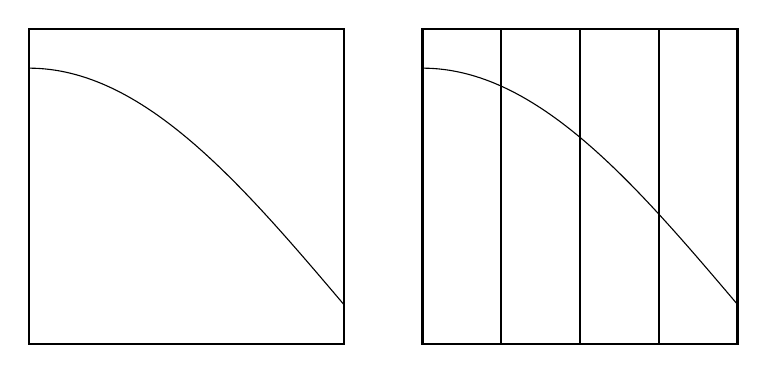
\begin{tikzpicture}
	\draw[thick] (0cm, 0cm) rectangle (4cm, 4cm);
	\foreach \x in {5cm, 6cm, 7cm, 8cm}
		\draw[thick] (\x, 0cm) rectangle (\x + 1 cm, 4cm);
	
	\draw (0,3.5) cos (4,0.5);
	\draw (5,3.5) cos (9,0.5);
	
\end{tikzpicture}
\caption{Wavelength and cell size}
\label{Wavelength-Vs-Cell-Size}
\end{figure}

% Reference for double figure: http://www.johndcook.com/blog/2009/01/14/how-to-display-side-by-side-figurs-in-latex/
\begin{figure}[H]
\centering
\mbox{\subfigure[Gaussian pulse of width 2]{\includegraphics[scale=0.4]{FigCh02_Pulsewidth2.png}}\quad\subfigure[Gaussian pulse of width 4]{\includegraphics[scale=0.4]{FigCh02_Pulsewidth4.png}}}\\
\mbox{\subfigure[Gaussian pulse of width 8]{\includegraphics[scale=0.4]{FigCh02_Pulsewidth8.png}}\quad\subfigure[Gaussian pulse of width 16]{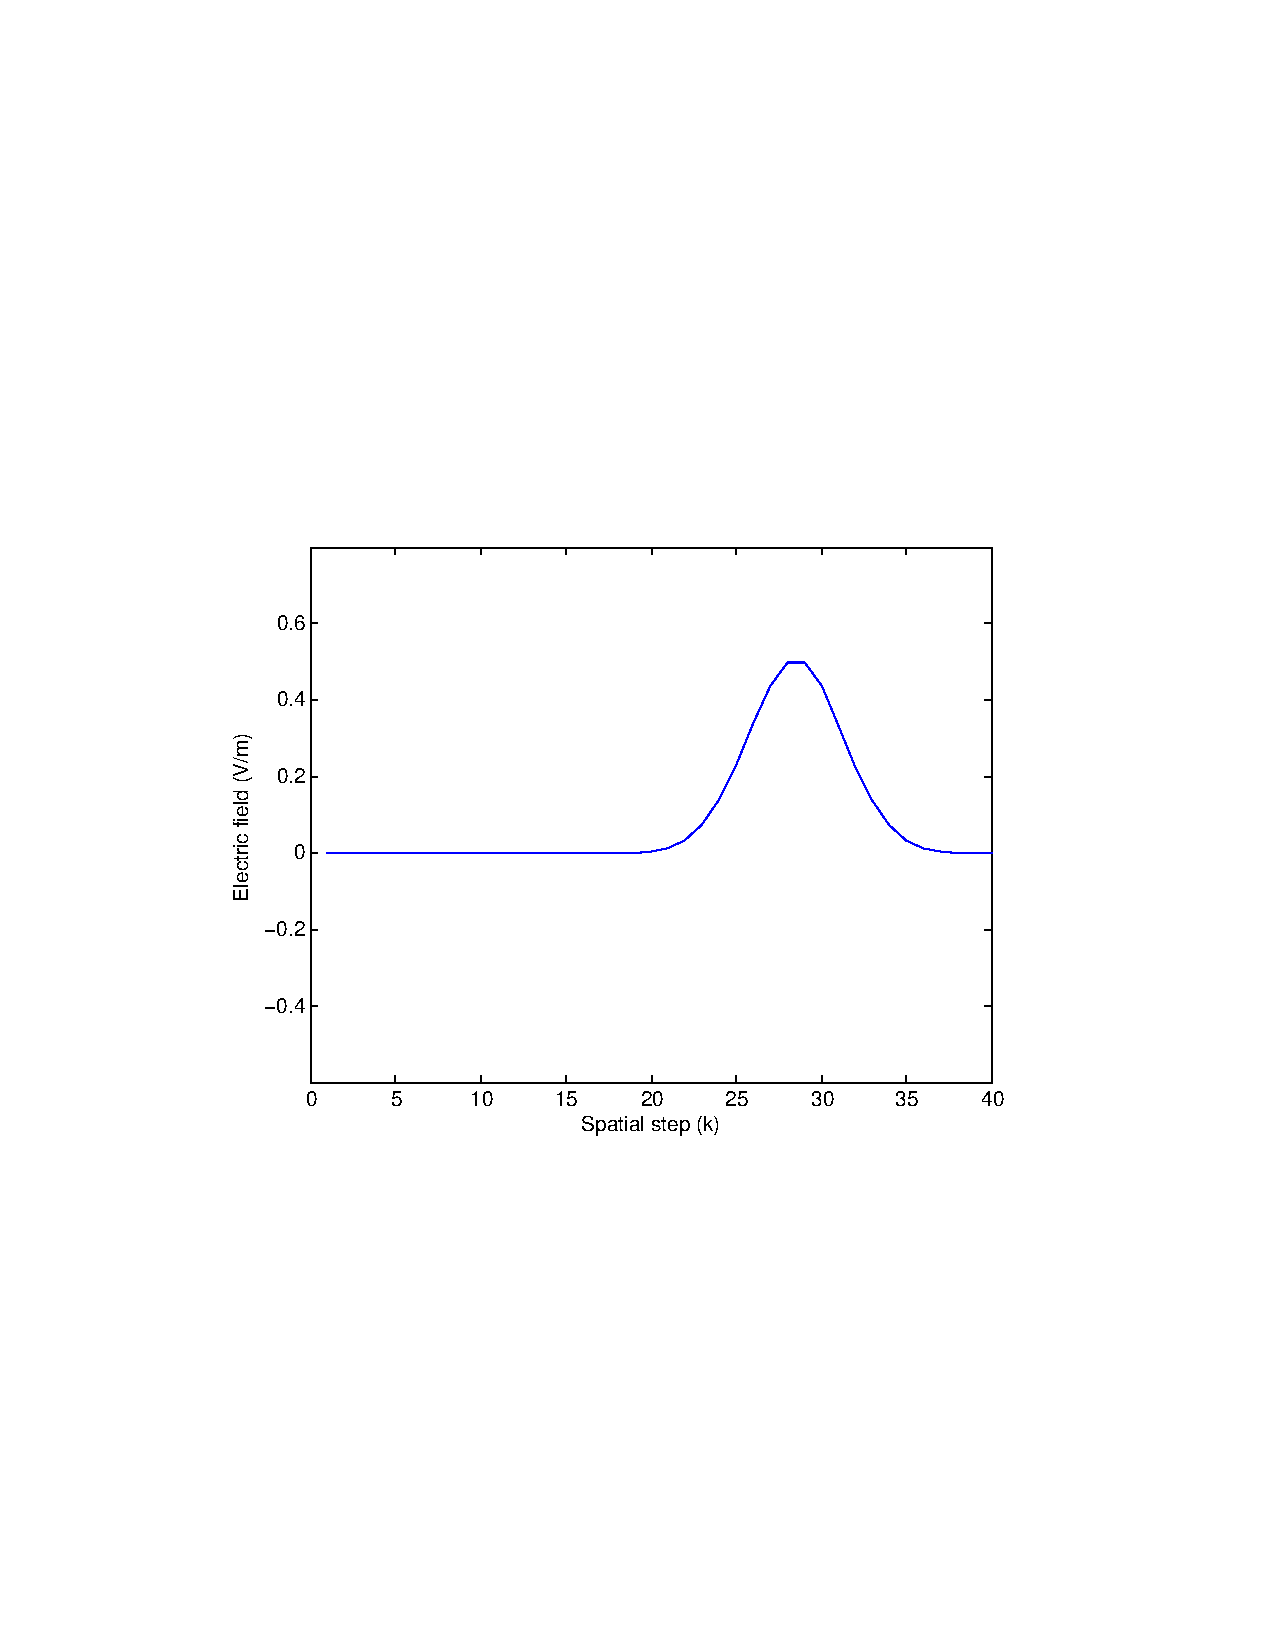
\includegraphics[scale=0.4]{FigCh02_Pulsewidth16.png}}}
\caption{Comparison of pulse width}
\label{Pulsewidth-comparison}
\end{figure}

\begin{figure}[H]
\centering
\mbox{\subfigure[$S_c = 1$]{\includegraphics[scale=0.4]{FigCh02_Stable1DFDTD.png}}\quad\subfigure[$S_c = 1.1$]{\includegraphics[scale=0.4]{FigCh02_Unstable1DFDTD.png}}}
\caption{$S_c$ and stability of FDTD}
\label{Unstable-FDTD}
\end{figure}
Inaccuracies may also result from inappropriate selection of spatial or time steps. Figure~\ref{Unstable-FDTD} shows that FDTD quickly becomes unstable if $S_c$ becomes greater than unity. Further to this, FDTD is inherently dispersive in nature and a pulse will spread as it travels over a period of time. While these inaccuracies cannot be completely eliminated, they can be reduced with proper selection of simulation parameters.

\section{Grid Termination and Boundary Conditions}
This section is a discussion on a number of grid termination conditions also known as boundary conditions. A graphical picture of different boundary conditions is given in figure~\ref{Boundary-Conditions}.
\subsection{Perfect Electric Conductor (PEC)}
Where electric field nodes are located at the outermost boundary these can be set to zero to simulate a PEC boundary. A wave incident on PEC will be completely reflected with a 180 degree phase shift.
\subsection{Perfect Magnetic Conductor (PMC)}
PMC is modelled by setting magnetic field nodes at edges set to zero. A PMC boundary will reflect incoming wave without any change in phase.
\subsection{Continuous Boundary Condition (CBC)}
In CBC incident waves will wrap around the and appear on the opposite edge. It is used to model the domain as a circular or continuous space. CBC boundary is implemented by incorporating the fields on edges in the FDTD update equations.
\subsection{Absorbing Boundary Condition (ABC)}
An ABC will completely absorb incident fields without any reflection. This is useful for antenna radiation and scattering problems. There are a number of techniques for modelling ABCs, most popular being perfectly matched layer or PML.

\begin{figure}[H]
\centering
\mbox{\subfigure[Incident wave]{\includegraphics[scale=0.2]{FigCh02_Incident_Wave.png}}\quad\subfigure[Reflection from PMC]{\includegraphics[scale=0.2]{FigCh02_PMC_Reflected.png}}}
\mbox{\subfigure[Incident wave]{\includegraphics[scale=0.2]{FigCh02_Incident_Wave.png}}\quad\subfigure[Reflection from PEC]{\includegraphics[scale=0.2]{FigCh02_PEC_Reflected.png}}}
\mbox{\subfigure[Incident wave]{\includegraphics[scale=0.2]{FigCh02_Incident_Wave.png}}\quad\subfigure[Continuous boundary (CBC)]{\includegraphics[scale=0.2]{FigCh02_CBC.png}}}
\mbox{\subfigure[Incident wave]{\includegraphics[scale=0.2]{FigCh02_Incident_Wave.png}}\quad\subfigure[Absorbing boundary (ABC)]{\includegraphics[scale=0.2]{FigCh02_ABC.png}}}
\caption{Boundary Conditions: Incident wave is moving towards right.}
\label{Boundary-Conditions}
\end{figure}

\chapter{FDTD Implementation of Metamaterials Using Dispersive Models}
\section{Limitations of Standard FDTD Algorithm}

\section{Using the Drude Dispersive Model}
Using Drude model values of plasma frequencies for regions corresponding to given values of $\epsilon$ and $\mu$ are specified. The FDTD methods requires some modification~\cite{Radial-Zhao}.

\chapter{FDTD Modelling of Lossless Cylindrical Cloak}
\section{Problem Specification}
\section{Matlab Implementation}
\section{C++ Implementation}

\chapter{GPU implementation}
\section{GPU Specifications}
\section{API Selection}
\section{Simulation Parameters}
\section{Memory Considerations}
\section{Thread Management}

\chapter{Conclusion}

\nocite{*}
\bibliographystyle{ieeetr} %plain, ieeetr
\bibliography{FDTD_Ref}

\appendix
\chapter{FDTD Code for 1D Wave Propagation in Free Space}
\begin{lstlisting}
% Simulation parameters.
SIZE = 512; % No. of spatial steps
MaxTime = 512; % No. of time steps
PulseWidth = 128; % Width of Gaussian Pulse
imp0 = 377.0; % Impedence of free space

% Constants.
c = 3e8;
pi = 3.141592654;
e0 = (1e-9)/(36*pi);
u0 = (1e-7)*4*pi;

dt = 1e-12;
dz = 3e-4;
Sc = c * dt/dz

% Initialization.
Ex = zeros ( SIZE, MaxTime ); % z-component of E-field
Hy = zeros ( SIZE, MaxTime ); % y-component of H-field
PLOT1(1) = 0; % Data for plotting.

% Outer loop for time-stepping.
tic
for q = 2:MaxTime
    % Calculation of Hy using update difference equation for Hy. This is time step q.
    Hy(1:SIZE-1,q) = Hy(1:SIZE-1,q-1) + ( ( Ex(1:SIZE-1,q-1) - Ex(2:SIZE,q-1) ) * dt/(u0*dz) );
    % ABC for H at SIZE.
    Hy(SIZE,q) = Hy(SIZE-1,q-1) + (Sc-1)/(Sc+1)*(Hy(SIZE-1,q) - Hy(SIZE,q-1) );
    
    % Calculation of Ez using updated difference equation for Ez. This is time step q+1/2.
    Ex(2:SIZE,q) = Ex(2:SIZE, q-1) + ( dt/(e0*dz)*(Hy(1:SIZE-1, q) - Hy(2:SIZE, q)) );
    % ABC for E at 1.
    Ex(1,q) = Ex(2,q-1) + (Sc-1)/(Sc+1)*(Ex(2,q) - Ex(2,q-1));
    
    % Activating a plane-wave source.
    Ex(100,q) = Ex(100,q) + exp( -1*(q-PulseWidth)^2/PulseWidth ) * Sc;
end
toc

% Simulation animation.
for i=1:MaxTime
    figure (2)
    plot ( Ex(:,i) )
end

\end{lstlisting}

\chapter{1D FDTD Demonstrating CBC}
\begin{lstlisting}
% Simulation parameters.
SIZE = 1024; % No. of spatial steps
MaxTime = 2024; % No. of time steps
imp0 = 377.0; % Impedence of free space

% Constants.
c = 3e8;
pi = 3.141592654;
e0 = (1e-9)/(36*pi);
u0 = (1e-7)*4*pi;

dt = 0.8e-12;
dx = 3e-4;
Sc = c * dt/dx

% Initialization.
Ez = zeros ( SIZE, MaxTime ); % z-component of E-field
Hy = zeros ( SIZE, MaxTime ); % y-component of H-field
PLOT1(1) = 0; % Data for plotting.

% Outer loop for time-stepping.
tic
for q = 2:MaxTime
    % Calculation of Hy using update difference equation for Hy. This is time step q.
    Hy(1:SIZE-1,q) = Hy(1:SIZE-1,q-1) + ( ( Ez(2:SIZE,q-1) - Ez(1:SIZE-1,q-1) ) * dt/(u0*dx) );
    % CBC for H at SIZE.
    Hy(SIZE,q) = Hy(SIZE,q-1) + ( ( Ez(1,q-1) - Ez(SIZE,q-1) ) * dt/(u0*dx) );
    
    % Calculation of Ez using updated difference equation for Ez. This is time step q+1/2.
    Ez(2:SIZE,q) = Ez(2:SIZE, q-1) + ( dt/(e0*dx)*(Hy(2:SIZE, q) - Hy(1:SIZE-1, q)) );
    % CBC for E at 1.
    Ez(1,q) = Ez(1,q-1) + ( dt/(e0*dx)*(Hy(1, q) - Hy(SIZE, q)) );
    
    % Activating a plane-wave source.
    Ez(100,q) = Ez(100,q) + exp( -1*((q-256)^2)/1000 ) * Sc;
end
toc

% Simulation animation.
for i=1:MaxTime
    figure (2)
    plot ( Ez(:,i) )
end

\end{lstlisting}

\end{document}




